% !TEX TS-program = xelatex
% !TEX encoding = UTF-8

% This is a simple template for a XeLaTeX document using the "article" class,
% with the fontspec package to easily select fonts.

\documentclass[11pt]{report} % use larger type; default would be 10pt
\usepackage{fontspec} % Font selection for XeLaTeX; see fontspec.pdf for documentation
\defaultfontfeatures{Mapping=tex-text} % to support TeX conventions like ``---''
\usepackage{xunicode} % Unicode support for LaTeX character names (accents, European chars, etc)
\usepackage{xltxtra} % Extra customizations for XeLaTeX
% \fontspec{"[DroidSerif.ttf]"}
% \setmainfont{Droid Serif} % set the main body font (\textrm), assumes Charis SIL is installed
%\setsansfont{Deja Vu Sans}
%\setmonofont{Deja Vu Mono}
\usepackage{amsmath}
\usepackage{xfrac}
% \usepackage{xfrac,unicode-math}
% \setmathfont[version=cambria]{Cambria Math}
% \mathversion{cambria}
\usepackage{cleveref}
\usepackage{epstopdf}
\usepackage{amsmath}
\usepackage{hyperref}
\usepackage{xspace}
\usepackage{mathtools}
\usepackage{tikz}
\usepackage{epsfig}
\usepackage{float}
\usepackage{natbib}
\usepackage{subfigure}
\usepackage{setspace}
\usepackage{tabularx,ragged2e,booktabs,caption}
\usepackage{wrapfig}

% other LaTeX packages.....
\usepackage{geometry} % See geometry.pdf to learn the layout options. There are lots.
\geometry{letterpaper} % or letterpaper (US) or a5paper or....
%\usepackage[parfill]{parskip} % Activate to begin paragraphs with an empty line rather than an indent

\usepackage{graphicx} % support the \includegraphics command and options
\newcommand{\IDK}{*** I DON'T KNOW THIS WORD***}
\newcolumntype{b}{X}
\newcolumntype{s}{>{\hsize=.2\hsize}X}

\title{237D Fusion Technology \\
Handout v. 9.2}
\author{Professor Mohamed Abdou}
%\date{} % Activate to display a given date or no date (if empty),
         % otherwise the current date is printed 


\begin{document}
\maketitle
\chapter{Radiation Shielding}
\section{Page 1}
\section{Page 2}
\subsection{Types of Shielding in Fusion Reactor}

\begin{itemize}
\item bulk shield (surrounding the blanket to protect vacuum vessel and superconducting magnets.
\item Penetration shield (around penetrations, e.g. natural beams, vacuum ducts)
\item Biological (reactor building walls, typically concrete; protect personnel in central rooms and outside.)
\end{itemize}

\section{Page 3}
\subsection{Bulk Shield}
This is a large component of fusion reactor. It is outside the blanket and inside the vacuum vessel.
\underline{Topics to be covered}
\begin{itemize}
\item Shield material composition
\item Radiation damage to superconducting magnet materials
\item Optimization of inboard blanket/shield thickness
\end{itemize}
\section{Page 4}
\begin{figure}[H]
  \centering
  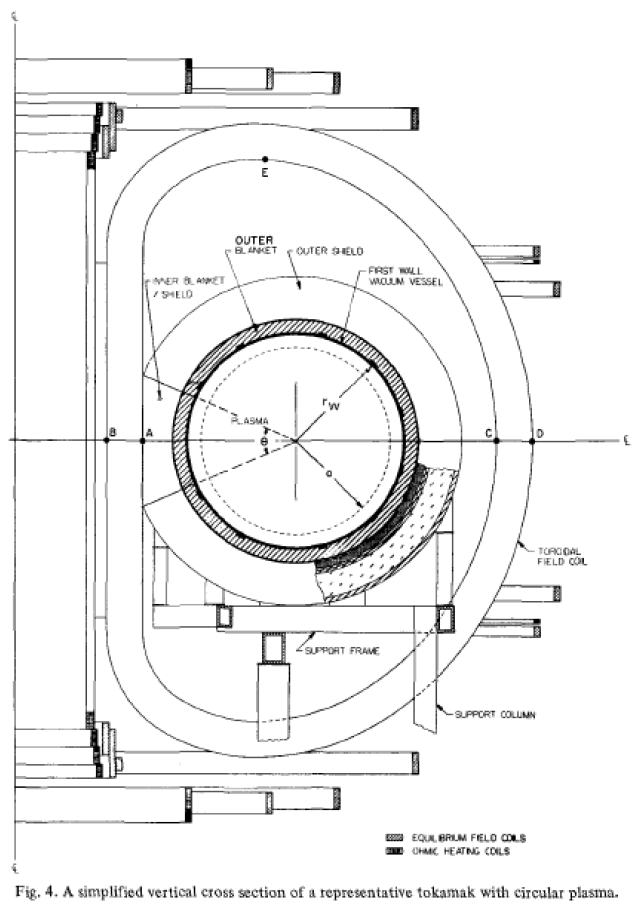
\includegraphics[width=0.45\textwidth]{figs/tokamak.png}
  \caption{A simplified vertical cross section of a representative tokamak with circular plasma.}
\end{figure}

\section{Page 5}
\subsection{Shield Composition}
A considerable fraction of the neutrons leaking from the blanket have kinetic energies above a few MeV. A basic requirement therefore of the shielding material is to have a large attenuation coefficient for high energy neutrons. Inevitably, this has to be a material of moderate of large mass number since inelastic scattering is the most efficient mechanism for reducing the energies of high energy neutrons. Furthermore, light materials such as water, LiH, and lithium have small total cross sections at high energies when compared with heavy materials. Stainless steel and lead have relatively large total cross sections above 3 MeV and the average secondary neutron energy per inelastic collision at 14 MeV is 2.2 and 2.5 MeV in lead and iron, respectively. Both materials are available, relatively inexpensive, and a great deal of knowledge about their characteristics exist. Below the inelastic threshold, however, these materials are no longer effective and a light material should be present. Borated water is efficient and is almost cost free. However, the presence of water in the same system with a high-temperature liquid metal increases significantly the hazard of accidental energy release. Graphite is an alternative choice. In addition, to minimize the gamma emission from radiative capture reactions, it is essential to use a sufficient amount of B$^10$ which has a large (n,$\alpha$) cross section for low energy neutrons and is associated with only soft gamma (0.5 MeV) emission (compared with a strong line at 7.6 MeV in the capture gamma ray spectrum for iron). Boron carbide B$_4$C irradiation but helium production is large. However, if B$_4$C is used in the shield with only 80\% of the theoretical density, the swelling problem due to the excessive helium production can be tolerated. Boral (50\% B$_4$C and 50\% Al) is another good choice.

Based on the above discussion, a mixture of stainless steel and boron carbide, or of lead and B$_4$C, or a combination of the three materials are reasonable choices and further investigation is needed to find the optimum composition and shield depth for an overall low cost. For this purpose, a fixed composition and configuration of the blanket coupled to a shield for which the parameters are to be varied as shown in figure FIGURE is considered. The blanket consists of a 1 cm first wall, 42 cm of 95\% Li plus 5\% structure. The first wall and blanket structure is niobium in the following calculations but the results in the shield are insensitive to this choice. The extra 7 m of lithium at the outer face of the reflector region was introduced to meet the cooling requirements of the reflector and inner regions of the shield. As preliminary criteria, the attenuation required in the blanket and shield should be roughly 10$^6$. This requirement can be satisfied by approximately 70 cm of stainless steel plus boron carbde following the blanket described above. As a starting point, figure FIGURE in which the blanket is followed by a one meter shield was considered as a reference design for investigating various aspects of the shield design. Six cases for the composition of the shield were considered; 70\% SS plus 30\% B$_4$C (design 114), 70\% Pb plus 30\% B$_4$C (design 115), 35\% SS plus 35\% Pb plus 30\% B$_4$C (design 115), 100\% SS (design 117), 85\% Pb + 15\% B$_4$ (design 118), and 50\%, where percentages are by volume. Neutronics and photonics calculations were carried out for the six designs. It has been shown REFERENCE that the convergence of the discrete ordinates results for such a system are achieved by S$_8$ and S$_4$ overestimates the leakage by 10 to 15\%. In order to reduce the cost for these calculations, S$_4$ was used. The comparison is not significantly affected by the difference between S$_4$ and S$_8$. Cylindrical geometry and the P$_3$ approximation of the scattering anisotropy were used in all calculations.

The energy leakage, L$_{TE}$, is plotted against the distance from the inner boundary of the shield for designs 114 through 117 in fig. FIGURE and for designs
\section{Page 6}
115, 118, and 119 in figure FIGURE. L$_{TE}$, is the sum of the neutron energy leakage, L$_{nE}$, and the gamma energy leakage, L$_{\gamma E}$, where L$_{nE}$ is defined in the multigroup representation at any surface of a one-dimensional cylinder as

\begin{equation}
  L_{nE}(r) = 2 \pi r \sum_g E_{ng} (r) J_{ng} (r)
\end{equation}

Where $J_{ng}$ is the (net) neutron current density at the surface in energy group $g$, and $E_{ng}$ is approximated by the midpoint energy of group $g$. Similar definitions apply for gammas with the subscript $\gamma$ replacing $n$. Since the energy deposition in the magnet by neutrons and photons streaming out of the shield increasing, in general, with the neutron and  photon energies we find it more meaningful in comparing the performance of various shield compositions to compare the “energy” rather than the “number” attenuations.
The results in figures FIGURES show that L$_{TE}$ varies exponentially with the spatial variable, $r$, i.e.

\begin{equation}
L_{TE} (r) = L_{TE} (r_0) e^{-\mu_t (r-t_0)}
\end{equation}

Where $\mu_t$ (with or without the subscript) is the total energy attenuation coefficient. Similar results were found for both the neutron and gamma fluxes i.e.

\begin{equation}
L_{nE} (r) = L_{nE} (r_0) e^{-\mu_n (r-t_0)}
\end{equation}
\begin{equation}
L_{\gamma E} (r) = L_{\gamma E} (r_0) e^{-\mu_{\gamma} (r-t_0)}
\end{equation}

The energy attenuation coefficients $\mu_n,\mu_{\gamma}$, and $\mu_t$ obtained for the six designs discussed above are given in table TABLE. Several conclusions can be reached from examining the attenuation curves of figures FIGURES and the energy attenuation coefficients in table TABLES: 1- Comparison of $L_{TE}$ for designs 114, 115 and 116 shows that stainless steel has considerably better attenuation characteristics than lead if both are mied with a fair amount of light material. 2- Comparison of $L_{TE}$ for designs 114 and 117 shows that the presence of B$_4$C (or an alternative) is necessary. At the end of a one meter shield the total energy leakage from a 100\% stainless steel shield is about two orders of magnitude higher than that from a shield consisting of 70\% SS plus 30\% B$_4$C. This is mainly due to two causes. B$_4$C is better than SS at attenuating neutrons below about 2 MeV. In addition, in the absence of B$^{10}$, neutrons slowed down eventually get absorbed in radiative capture reactions in stainless steel increasing the gamma energy production. 3- Figure FIGURE which compares L$_{TE}$ for 85\% Pb + 15\% B$_4$C, 70\% Pb + 30\% B$_4$C, and 50\% Pb + 50\% B$_4$C shows that increasing the volume percentage of B$_4$C to 50\% (and probably higher) improves the attenuation considerably. If other light materials such as graphite or water are used, the optimal volume percentages are usually much less (roughly 30\%) than that for B$_4$C. 4- Although lead is more efficient in attenuating gamma radiation, we found that using stainless steel does not increase the gamma energy leakage, $L_{\gamma E}$, appreciably. Furthermore, table TABLE shows that $\mu_{\gamma}$ is greater in stainless steel-B$_4$C than in Pb-B$_4$C mixtures. These results can be explained as follows. The photons in the shield come primarily from gammas produced by neutron interactions in the shield rather than by penetration from the blanket. Stainless steel attenuates fast neutrons quickly in the first few mean free paths, thus the photons produced have a long distance in which to be absorbed. In addition, the gamma energy leakage in the outer regions is affected most by the gammas produced in these regions. The seconday gama production in deeper regions of a SS-B$_4$C shield is significantly lower than in the same regions of the Pb-B$_4$C shield.

\subsection{Optimization of a Shield Thickness}
Increasing the thickness of a shield increases its cost and the magnet
\section{Page 7}
\begin{figure}[H]
  \centering
  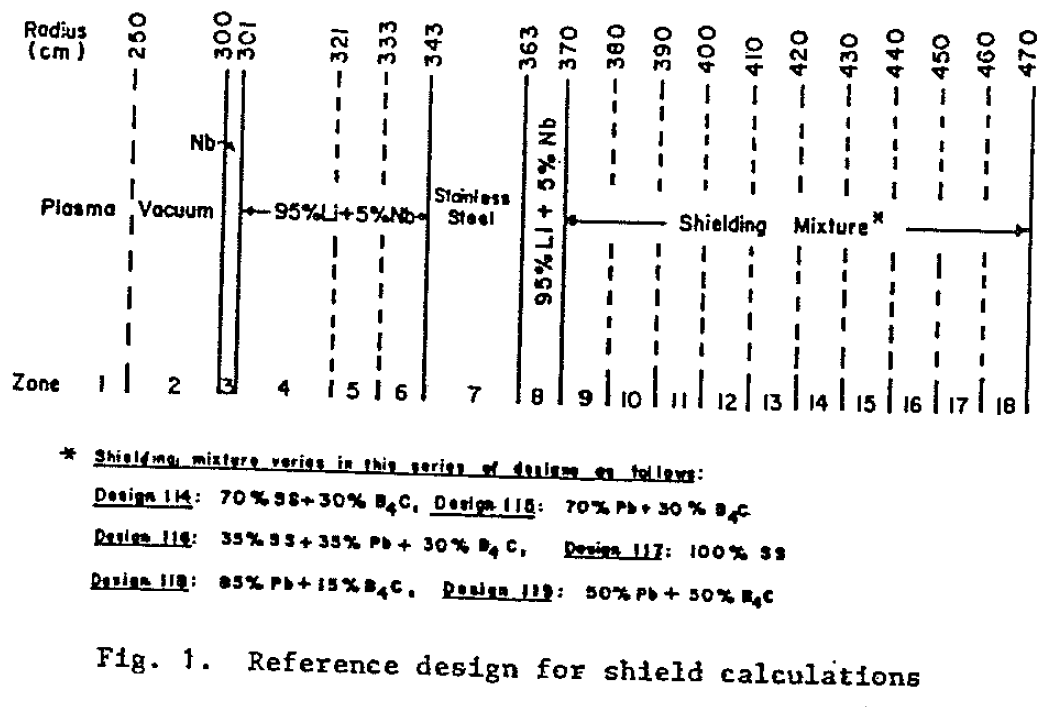
\includegraphics[width=0.45\textwidth]{figs/shield.png}
  \caption{Reference design for shield calculations.}
\end{figure}

\begin{figure}[H]
  \centering
  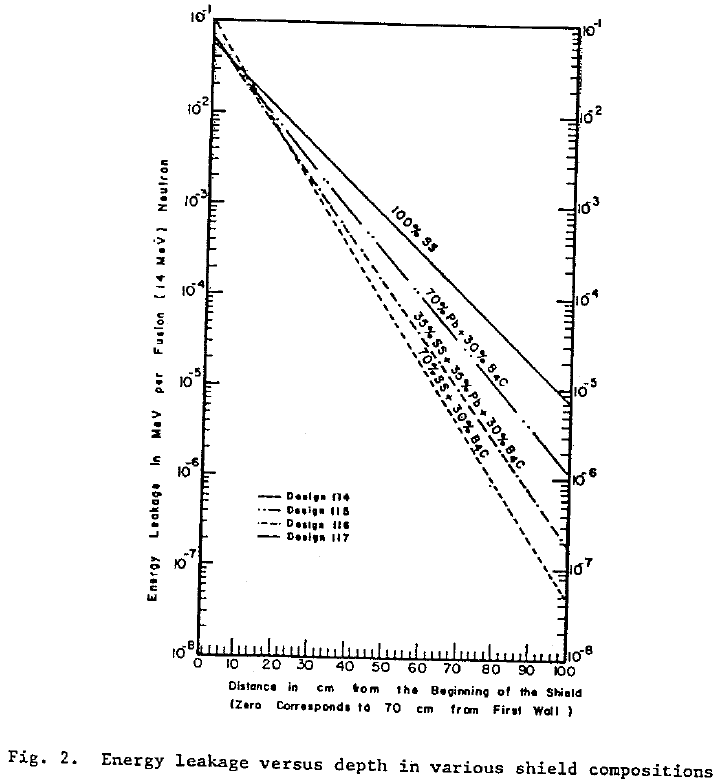
\includegraphics[width=0.45\textwidth]{figs/energyLeakage.png}
  \caption{Energy leakage versus depth in various shield compositions.}
\end{figure}

\section{Page 8}
\begin{table}
\begin{tabularx}{\textwidth}{|b|s|s|s|s|s|s|}
\hline
Design ID & 114 & 115 & 116 & 117 & 118 & 119 \\
\hline
Shield Composition (all percentages are by volume)  &
  70\% SS + 30\% B$_4$C                             &
  70\% Pb + 30\% B$_4$C                             &
  35\% Pb + 35\% SS + 30\% B$_4$C                   &
  100\% SS                                          &
  85\% Pb + 15\% B$_4$C                             &
  50\% Pb + 50\% B$_4$C                             \\
  \hline
Neutron Energy Attenuatuion Coefficient, $\mu_n$ (cm$^{-1}$) &
 0.1438 & 0.1113 & 0.1282 & 0.1022 & 0.0977 & 0.1161  \\
  \hline
Gamma Energy Attenuation Coefficient, $\mu_{\gamma}$ (cm$^{-1}$) &
 0.1466  & 0.1160 & 0.1320  & 0.0828  & 0.1008  & 0.1190 \\
  \hline
Total Energy Attenuation Coefficient, $\mu_{t}$ (cm$^{-1}$) &
0.1445 & 0.1113 & 0.1283 & 0.0902 & 0.0976 & 0.1161 \\
\hline
\end{tabularx}
\caption{Neutron, Carma, and Total Energy Attenuation Coefficients$^*$ for Various Shield Compositions} \label{tab:attenuationCoeffs}
\end{table}
$^*$ obtained by fitting the energy attenuation curves to exponentials (see Text)

\section{Page 9}
\begin{figure}[H]
  \centering
  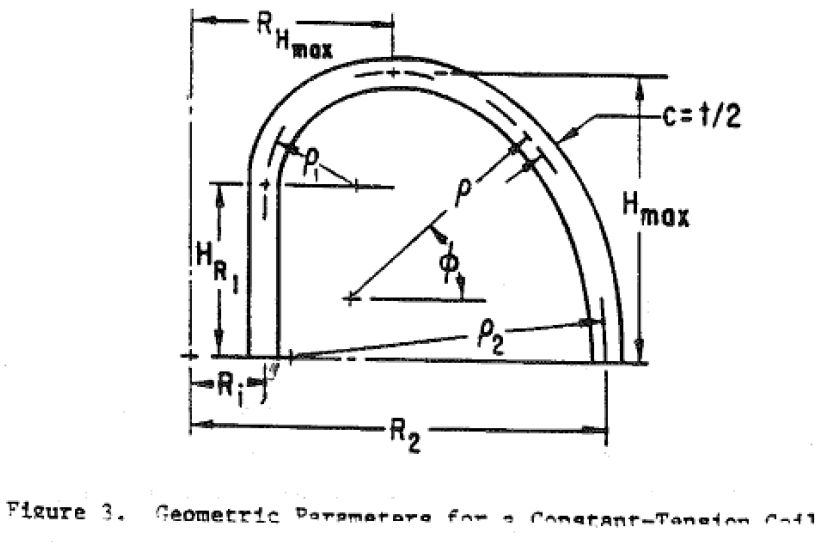
\includegraphics[width=0.45\textwidth]{figs/geometricParams.png}
  \caption{Geometric Parameters for a Constant \IDK.}
\end{figure}

\section{Page 10}
\begin{figure}[H]
  \centering
  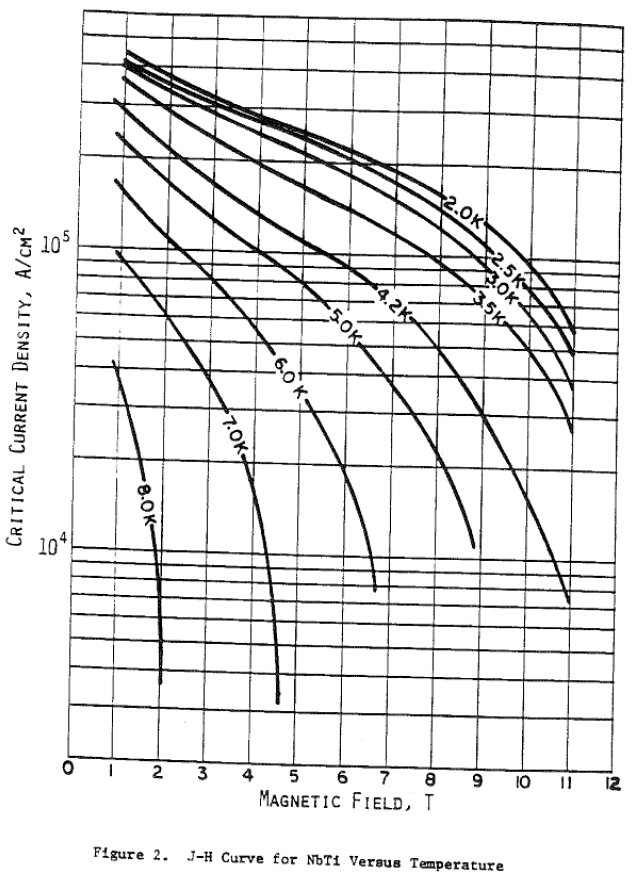
\includegraphics[width=0.45\textwidth]{figs/CriticalCurrent.png}
  \caption{J-H Curve for NbTi Versus Temperature.}
\end{figure}

\section{Page 11,12,13}
These pages were already in handout 9.

\section{Page 14}
\subsection{Optimization of Inboard Blanket and Shield Thickness in Tokamak}
\underline{Tradeoffs between:}
\begin{itemize}
\item Reactor size, reactor power, magnetic field, etc.
\item Protection of S.C. Magnet
\end{itemize}
\section{Page 15}
\subsection{Motives for Larger Blanket and Shield Thickness}
\underline{Shield Function}: Radiation protextion of S.C. magnet

\begin{equation}
\phi_m \sim \phi_w e^{-\mu \Delta_{BS}^i}
\end{equation}


\begin{align}
\phi_w & = \text{flux at first wall (fixed by design)}
\mu & = \text{attenuation coefficient (fixed by shielding composition)}
\end{align}

\underline{Magnet Protection}
\begin{itemize}
\item Refrigeration power requirements
\item Change in superconductor $J_c,T_c$
\item Radiation-induced resistivity in stabilizer
\item Change in mechanical and dielectric properties of insulators
\end{itemize}

\section{Page 16}
\subsection{Motive for Smaller Blanket / Shield Thickness}


\end{document}
